\section{Remoção}

\begin{frame}[fragile]{Remoção do início}

    \begin{itemize}
        \item A remoção de um elemento do início de uma lista duplamente encadeada
        (\code{c++}{pop_front()}) tem complexidade $O(1)$

        \item O primeiro passo da remoção é armazenar o membro \code{cpp}{head} em uma 
            variável temporária

        \item Em seguida, o membro \code{c++}{head} deve apontar para o próximo elemento da
            lista

        \item O membro \code{c}{next} de \code{c}{head} deve ser atualizado com o valor nulo,
            caso exista

        \item Por fim, o ponteiro armazenado na variável temporária é deletado

        \item O membro \code{c++}{size} deve ser decrementado, se existir

        \item \textit{Corner case:} a tentativa de remoção em uma lista vazia deve ser tratada
            de alguma maneira (código de erro, exceção, etc.)

        \item \textit{Corner case:} se a lista tiver exatamente um nó no momento da remoção,
            o membro \code{c++}{tail} deve receber o valor nulo
    \end{itemize}

\end{frame}

\begin{frame}[fragile]{Visualização da remoção no início da lista}

    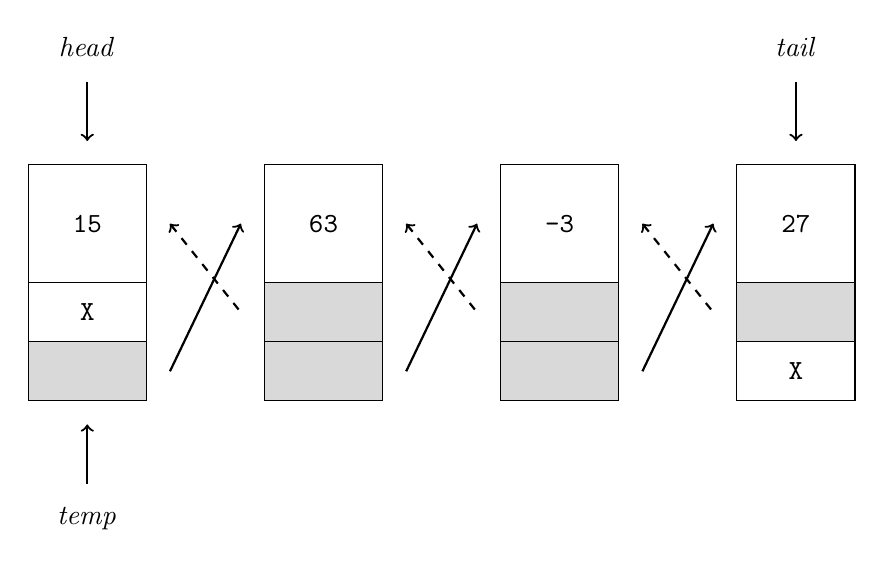
\begin{tikzpicture}[scale=1.5]
        \node[anchor=center] at (0.5, 3) {\textit{head}};
        \draw[->,thick] (0.5, 2.7) -- (0.5, 2.2);

        \node[anchor=center] at (6.5, 3) {\textit{tail}};
        \draw[->,thick] (6.5, 2.7) -- (6.5, 2.2);

        \node[anchor=center] at (0.5, -1) {\textit{temp}};
        \draw[->,thick] (0.5, -0.7) -- (0.5, -0.2);

        \draw[fill=white] (0,1) rectangle (1,2);
        \draw[fill=gray!30] (0,0) rectangle (1,0.5);
        \draw[fill=white] (0,0.5) rectangle (1,1);
        \node at (0.5,1.5) {\texttt{15}};
        \node at (0.5,0.75) {\textbf{\texttt{X}}};

        \draw[->,thick] (1.2, 0.25) -- (1.8, 1.5);
        \draw[<-,thick,dashed] (1.2, 1.5) -- (1.8, 0.75);

        \draw[fill=white] (2,1) rectangle (3,2);
        \draw[fill=gray!30] (2,0) rectangle (3,0.5);
        \draw[fill=gray!30] (2,0.5) rectangle (3,1);
        \node at (2.5,1.5) {\texttt{63}};

        \draw[->,thick] (3.2, 0.25) -- (3.8, 1.5);
        \draw[<-,thick,dashed] (3.2, 1.5) -- (3.8, 0.75);

        \draw[fill=white] (4,1) rectangle (5,2);
        \draw[fill=gray!30] (4,0) rectangle (5,0.5);
        \draw[fill=gray!30] (4,0.5) rectangle (5,1);
        \node at (4.5,1.5) {\texttt{-3}};

        \draw[->,thick] (5.2, 0.25) -- (5.8, 1.5);
        \draw[<-,thick,dashed] (5.2, 1.5) -- (5.8, 0.75);

        \draw[fill=white] (6,1) rectangle (7,2);
        \draw (6,0) rectangle (7,0.5);
        \draw[fill=gray!30] (6,0.5) rectangle (7,1);
        \node at (6.5,1.5) {\texttt{27}};
        \node at (6.5,0.25) {\textbf{\texttt{X}}};

    \end{tikzpicture}

\end{frame}

\begin{frame}[fragile]{Visualização da remoção no início da lista}

    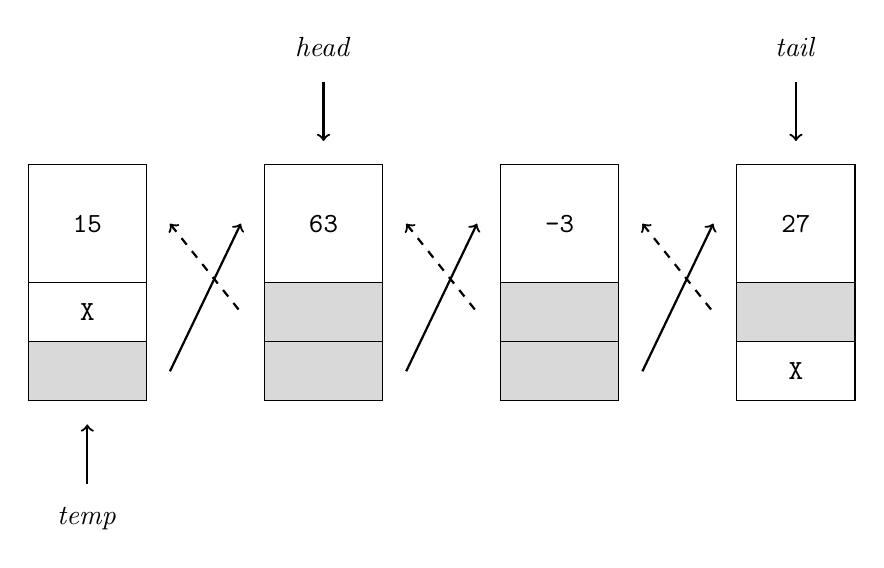
\begin{tikzpicture}[scale=1.5]
        \node[anchor=center] at (2.5, 3) {\textit{head}};
        \draw[->,thick] (2.5, 2.7) -- (2.5, 2.2);

        \node[anchor=center] at (6.5, 3) {\textit{tail}};
        \draw[->,thick] (6.5, 2.7) -- (6.5, 2.2);

        \node[anchor=center] at (0.5, -1) {\textit{temp}};
        \draw[->,thick] (0.5, -0.7) -- (0.5, -0.2);

        \draw[fill=white] (0,1) rectangle (1,2);
        \draw[fill=gray!30] (0,0) rectangle (1,0.5);
        \draw[fill=white] (0,0.5) rectangle (1,1);
        \node at (0.5,1.5) {\texttt{15}};
        \node at (0.5,0.75) {\textbf{\texttt{X}}};

        \draw[->,thick] (1.2, 0.25) -- (1.8, 1.5);
        \draw[<-,thick,dashed] (1.2, 1.5) -- (1.8, 0.75);

        \draw[fill=white] (2,1) rectangle (3,2);
        \draw[fill=gray!30] (2,0) rectangle (3,0.5);
        \draw[fill=gray!30] (2,0.5) rectangle (3,1);
        \node at (2.5,1.5) {\texttt{63}};

        \draw[->,thick] (3.2, 0.25) -- (3.8, 1.5);
        \draw[<-,thick,dashed] (3.2, 1.5) -- (3.8, 0.75);

        \draw[fill=white] (4,1) rectangle (5,2);
        \draw[fill=gray!30] (4,0) rectangle (5,0.5);
        \draw[fill=gray!30] (4,0.5) rectangle (5,1);
        \node at (4.5,1.5) {\texttt{-3}};

        \draw[->,thick] (5.2, 0.25) -- (5.8, 1.5);
        \draw[<-,thick,dashed] (5.2, 1.5) -- (5.8, 0.75);

        \draw[fill=white] (6,1) rectangle (7,2);
        \draw (6,0) rectangle (7,0.5);
        \draw[fill=gray!30] (6,0.5) rectangle (7,1);
        \node at (6.5,1.5) {\texttt{27}};
        \node at (6.5,0.25) {\textbf{\texttt{X}}};

    \end{tikzpicture}

\end{frame}

\begin{frame}[fragile]{Visualização da remoção no início da lista}

    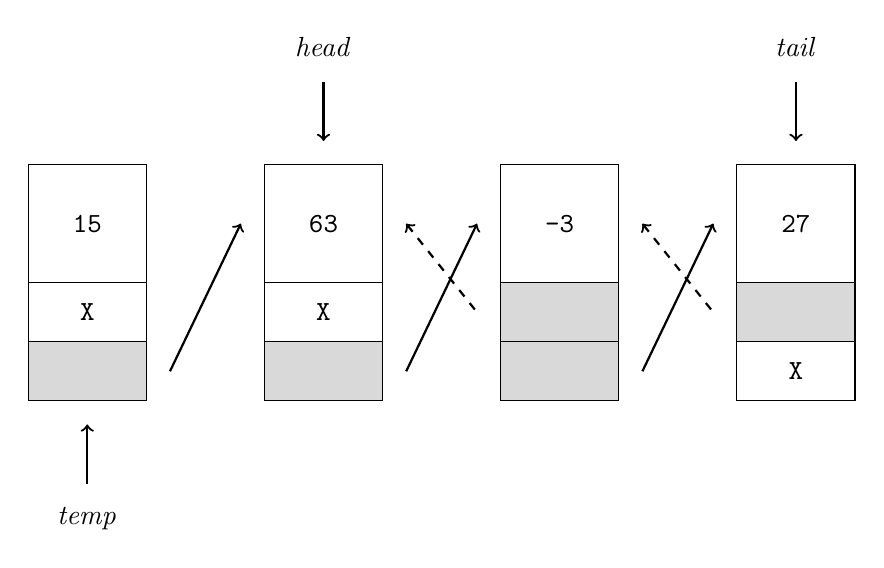
\begin{tikzpicture}[scale=1.5]
        \node[anchor=center] at (2.5, 3) {\textit{head}};
        \draw[->,thick] (2.5, 2.7) -- (2.5, 2.2);

        \node[anchor=center] at (6.5, 3) {\textit{tail}};
        \draw[->,thick] (6.5, 2.7) -- (6.5, 2.2);

        \node[anchor=center] at (0.5, -1) {\textit{temp}};
        \draw[->,thick] (0.5, -0.7) -- (0.5, -0.2);

        \draw[fill=white] (0,1) rectangle (1,2);
        \draw[fill=gray!30] (0,0) rectangle (1,0.5);
        \draw[fill=white] (0,0.5) rectangle (1,1);
        \node at (0.5,1.5) {\texttt{15}};
        \node at (0.5,0.75) {\textbf{\texttt{X}}};

        \draw[->,thick] (1.2, 0.25) -- (1.8, 1.5);

        \draw[fill=white] (2,1) rectangle (3,2);
        \draw[fill=gray!30] (2,0) rectangle (3,0.5);
        \draw[fill=white] (2,0.5) rectangle (3,1);
        \node at (2.5,1.5) {\texttt{63}};
        \node at (2.5,0.75) {\textbf{\texttt{X}}};

        \draw[->,thick] (3.2, 0.25) -- (3.8, 1.5);
        \draw[<-,thick,dashed] (3.2, 1.5) -- (3.8, 0.75);

        \draw[fill=white] (4,1) rectangle (5,2);
        \draw[fill=gray!30] (4,0) rectangle (5,0.5);
        \draw[fill=gray!30] (4,0.5) rectangle (5,1);
        \node at (4.5,1.5) {\texttt{-3}};

        \draw[->,thick] (5.2, 0.25) -- (5.8, 1.5);
        \draw[<-,thick,dashed] (5.2, 1.5) -- (5.8, 0.75);

        \draw[fill=white] (6,1) rectangle (7,2);
        \draw (6,0) rectangle (7,0.5);
        \draw[fill=gray!30] (6,0.5) rectangle (7,1);
        \node at (6.5,1.5) {\texttt{27}};
        \node at (6.5,0.25) {\textbf{\texttt{X}}};

    \end{tikzpicture}

\end{frame}

\begin{frame}[fragile]{Visualização da remoção no início da lista}

    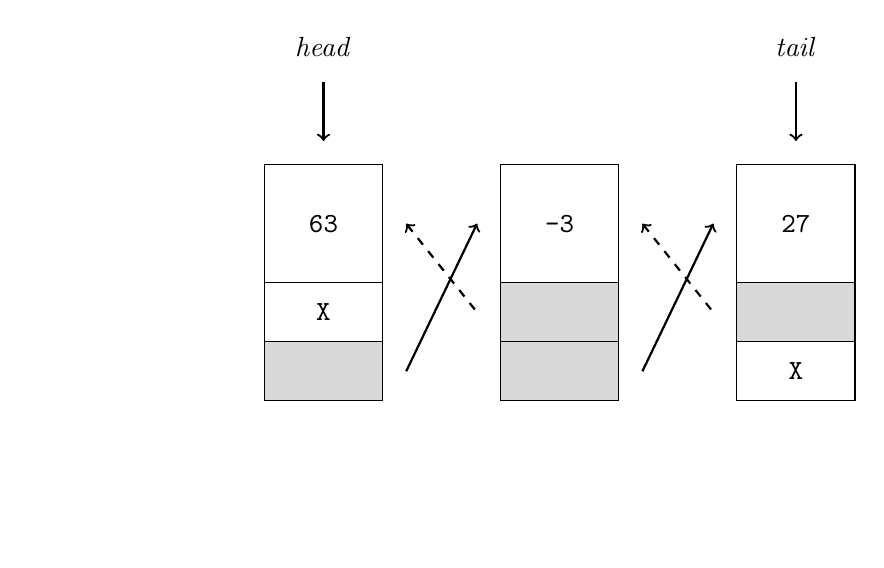
\begin{tikzpicture}[scale=1.5]
        \node[anchor=center] at (2.5, 3) {\textit{head}};
        \draw[->,thick] (2.5, 2.7) -- (2.5, 2.2);

        \node[anchor=center] at (6.5, 3) {\textit{tail}};
        \draw[->,thick] (6.5, 2.7) -- (6.5, 2.2);

        \node[white,anchor=center] at (0.5, -1) {\textit{temp}};
        \draw[white,->,thick] (0.5, -0.7) -- (0.5, -0.2);

        \draw[white] (0,1) rectangle (1,2);
        \draw[white] (0,0) rectangle (1,0.5);
        \draw[white] (0,0.5) rectangle (1,1);
        \node[white] at (0.5,1.5) {\texttt{15}};
        \node[white] at (0.5,0.75) {\textbf{\texttt{X}}};


        \draw[fill=white] (2,1) rectangle (3,2);
        \draw[fill=gray!30] (2,0) rectangle (3,0.5);
        \draw[fill=white] (2,0.5) rectangle (3,1);
        \node at (2.5,1.5) {\texttt{63}};
        \node at (2.5,0.75) {\textbf{\texttt{X}}};

        \draw[->,thick] (3.2, 0.25) -- (3.8, 1.5);
        \draw[<-,thick,dashed] (3.2, 1.5) -- (3.8, 0.75);

        \draw[fill=white] (4,1) rectangle (5,2);
        \draw[fill=gray!30] (4,0) rectangle (5,0.5);
        \draw[fill=gray!30] (4,0.5) rectangle (5,1);
        \node at (4.5,1.5) {\texttt{-3}};

        \draw[->,thick] (5.2, 0.25) -- (5.8, 1.5);
        \draw[<-,thick,dashed] (5.2, 1.5) -- (5.8, 0.75);

        \draw[fill=white] (6,1) rectangle (7,2);
        \draw (6,0) rectangle (7,0.5);
        \draw[fill=gray!30] (6,0.5) rectangle (7,1);
        \node at (6.5,1.5) {\texttt{27}};
        \node at (6.5,0.25) {\textbf{\texttt{X}}};

    \end{tikzpicture}

\end{frame}

\begin{frame}[fragile]{Implementação da remoção do início}
    \inputsnippet{c++}{59}{70}{list.h}
\end{frame}

\begin{frame}[fragile]{Remoção do final da lista}

    \begin{itemize}
        \item Mesmo com o membro \code{c++}{tail}, a remoção do último elemento de uma lista
            encadeada (\code{c++}{pop_back()}) tem complexidade $O(N)$, onde $N$ é o número de 
            nós da lista

        \item Isto acontece porque é preciso localizar o elemento que antecede o último elemento
        (\code{c++}{prev}), processo que tem complexidade linear

        \item Localizado o elemento \code{c}{prev}, a remoção é semelhante à remoção do início:
        o elemento \code{c++}{tail} é deletado e \code{c++}{tail} passa a apontar para
        \code{c++}{prev}

        \item Por fim, o membro \code{c++}{next} de \code{c++}{prev} deve se tornar nulo

        \item Novamente, o membro \code{c++}{size} deve ser decrementado, se existir

        \item \textit{Corner case:} lista vazia

        \item \textit{Corner case:} se a lista tiver exatamente um nó no momento da remoção,
            o membro \code{c++}{head} deve receber o valor nulo
    \end{itemize}

\end{frame}

\begin{frame}[fragile]{Visualização da remoção no final da lista}

    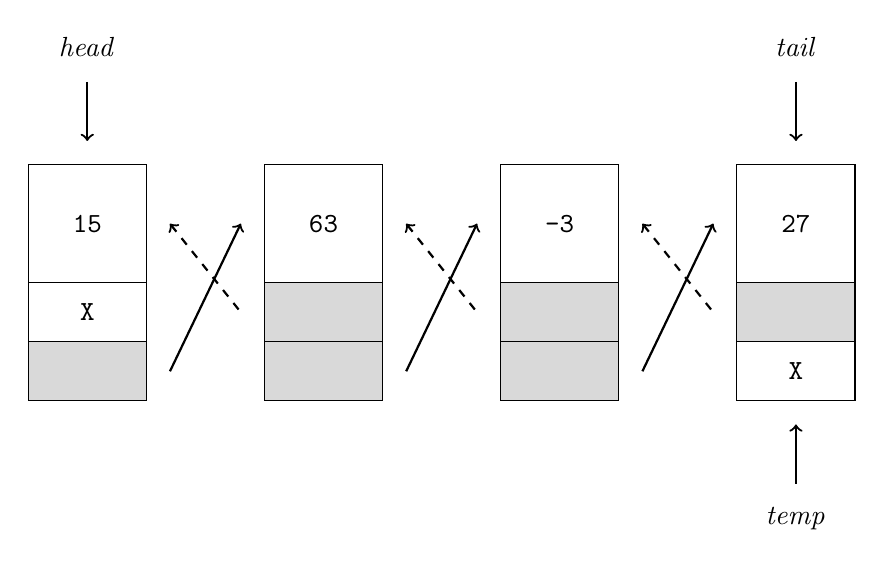
\begin{tikzpicture}[scale=1.5]
        \node[anchor=center] at (0.5, 3) {\textit{head}};
        \draw[->,thick] (0.5, 2.7) -- (0.5, 2.2);

        \node[anchor=center] at (6.5, 3) {\textit{tail}};
        \draw[->,thick] (6.5, 2.7) -- (6.5, 2.2);

        \node[anchor=center] at (6.5, -1) {\textit{temp}};
        \draw[->,thick] (6.5, -0.7) -- (6.5, -0.2);

        \draw[fill=white] (0,1) rectangle (1,2);
        \draw[fill=white] (0,0.5) rectangle (1,1);
        \draw[fill=gray!30] (0,0) rectangle (1,0.5);
        \node at (0.5,1.5) {\texttt{15}};
        \node at (0.5,0.75) {\textbf{\texttt{X}}};

        \draw[->,thick] (1.2, 0.25) -- (1.8, 1.5);
        \draw[<-,thick,dashed] (1.2, 1.5) -- (1.8, 0.75);

        \draw[fill=white] (2,1) rectangle (3,2);
        \draw[fill=gray!30] (2,0) rectangle (3,0.5);
        \draw[fill=gray!30] (2,0.5) rectangle (3,1);
        \node at (2.5,1.5) {\texttt{63}};

        \draw[->,thick] (3.2, 0.25) -- (3.8, 1.5);
        \draw[<-,thick,dashed] (3.2, 1.5) -- (3.8, 0.75);

        \draw[fill=white] (4,1) rectangle (5,2);
        \draw[fill=gray!30] (4,0) rectangle (5,0.5);
        \draw[fill=gray!30] (4,0.5) rectangle (5,1);
        \node at (4.5,1.5) {\texttt{-3}};

        \draw[->,thick] (5.2, 0.25) -- (5.8, 1.5);
        \draw[<-,thick,dashed] (5.2, 1.5) -- (5.8, 0.75);

        \draw[fill=white] (6,1) rectangle (7,2);
        \draw[fill=gray!30] (6,0.5) rectangle (7,1);
        \draw (6,0) rectangle (7,0.5);
        \node at (6.5,1.5) {\texttt{27}};
        \node at (6.5,0.25) {\textbf{\texttt{X}}};

    \end{tikzpicture}

\end{frame}

\begin{frame}[fragile]{Visualização da remoção no final da lista}

    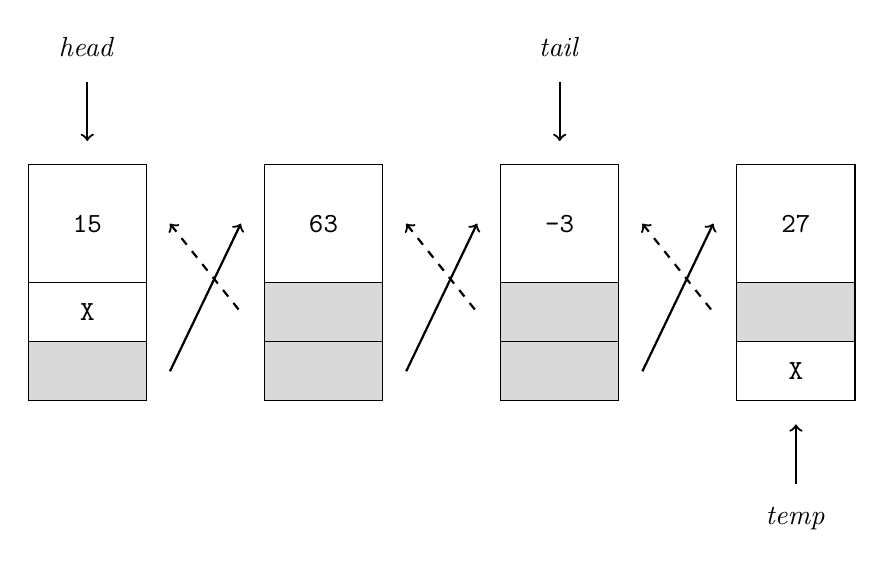
\begin{tikzpicture}[scale=1.5]
        \node[anchor=center] at (0.5, 3) {\textit{head}};
        \draw[->,thick] (0.5, 2.7) -- (0.5, 2.2);

        \node[anchor=center] at (4.5, 3) {\textit{tail}};
        \draw[->,thick] (4.5, 2.7) -- (4.5, 2.2);

        \node[anchor=center] at (6.5, -1) {\textit{temp}};
        \draw[->,thick] (6.5, -0.7) -- (6.5, -0.2);

        \draw[fill=white] (0,1) rectangle (1,2);
        \draw[fill=white] (0,0.5) rectangle (1,1);
        \draw[fill=gray!30] (0,0) rectangle (1,0.5);
        \node at (0.5,1.5) {\texttt{15}};
        \node at (0.5,0.75) {\textbf{\texttt{X}}};

        \draw[->,thick] (1.2, 0.25) -- (1.8, 1.5);
        \draw[<-,thick,dashed] (1.2, 1.5) -- (1.8, 0.75);

        \draw[fill=white] (2,1) rectangle (3,2);
        \draw[fill=gray!30] (2,0) rectangle (3,0.5);
        \draw[fill=gray!30] (2,0.5) rectangle (3,1);
        \node at (2.5,1.5) {\texttt{63}};

        \draw[->,thick] (3.2, 0.25) -- (3.8, 1.5);
        \draw[<-,thick,dashed] (3.2, 1.5) -- (3.8, 0.75);

        \draw[fill=white] (4,1) rectangle (5,2);
        \draw[fill=gray!30] (4,0) rectangle (5,0.5);
        \draw[fill=gray!30] (4,0.5) rectangle (5,1);
        \node at (4.5,1.5) {\texttt{-3}};

        \draw[->,thick] (5.2, 0.25) -- (5.8, 1.5);
        \draw[<-,thick,dashed] (5.2, 1.5) -- (5.8, 0.75);

        \draw[fill=white] (6,1) rectangle (7,2);
        \draw[fill=gray!30] (6,0.5) rectangle (7,1);
        \draw (6,0) rectangle (7,0.5);
        \node at (6.5,1.5) {\texttt{27}};
        \node at (6.5,0.25) {\textbf{\texttt{X}}};

    \end{tikzpicture}

\end{frame}

\begin{frame}[fragile]{Visualização da remoção no final da lista}

    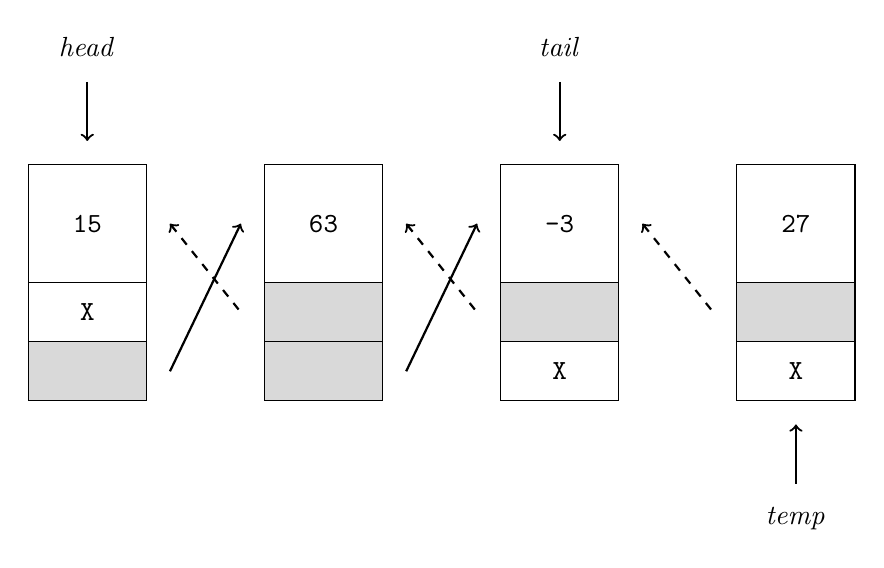
\begin{tikzpicture}[scale=1.5]
        \node[anchor=center] at (0.5, 3) {\textit{head}};
        \draw[->,thick] (0.5, 2.7) -- (0.5, 2.2);

        \node[anchor=center] at (4.5, 3) {\textit{tail}};
        \draw[->,thick] (4.5, 2.7) -- (4.5, 2.2);

        \node[anchor=center] at (6.5, -1) {\textit{temp}};
        \draw[->,thick] (6.5, -0.7) -- (6.5, -0.2);

        \draw[fill=white] (0,1) rectangle (1,2);
        \draw[fill=white] (0,0.5) rectangle (1,1);
        \draw[fill=gray!30] (0,0) rectangle (1,0.5);
        \node at (0.5,1.5) {\texttt{15}};
        \node at (0.5,0.75) {\textbf{\texttt{X}}};

        \draw[->,thick] (1.2, 0.25) -- (1.8, 1.5);
        \draw[<-,thick,dashed] (1.2, 1.5) -- (1.8, 0.75);

        \draw[fill=white] (2,1) rectangle (3,2);
        \draw[fill=gray!30] (2,0) rectangle (3,0.5);
        \draw[fill=gray!30] (2,0.5) rectangle (3,1);
        \node at (2.5,1.5) {\texttt{63}};

        \draw[->,thick] (3.2, 0.25) -- (3.8, 1.5);
        \draw[<-,thick,dashed] (3.2, 1.5) -- (3.8, 0.75);

        \draw[fill=white] (4,1) rectangle (5,2);
        \draw[fill=white] (4,0) rectangle (5,0.5);
        \draw[fill=gray!30] (4,0.5) rectangle (5,1);
        \node at (4.5,1.5) {\texttt{-3}};
        \node at (4.5,0.25) {\textbf{\texttt{X}}};

        \draw[<-,thick,dashed] (5.2, 1.5) -- (5.8, 0.75);

        \draw[fill=white] (6,1) rectangle (7,2);
        \draw[fill=gray!30] (6,0.5) rectangle (7,1);
        \draw (6,0) rectangle (7,0.5);
        \node at (6.5,1.5) {\texttt{27}};
        \node at (6.5,0.25) {\textbf{\texttt{X}}};

    \end{tikzpicture}

\end{frame}

\begin{frame}[fragile]{Visualização da remoção no final da lista}

    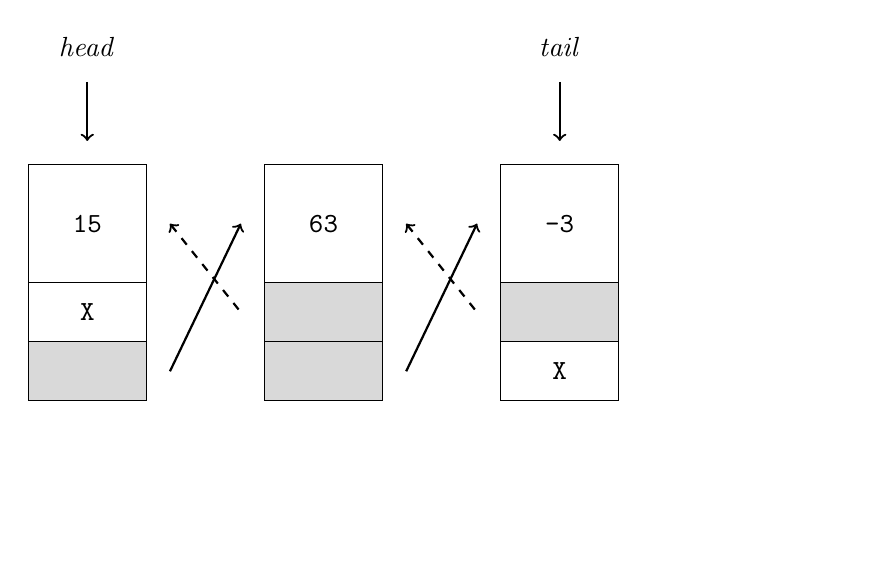
\begin{tikzpicture}[scale=1.5]
        \node[anchor=center] at (0.5, 3) {\textit{head}};
        \draw[->,thick] (0.5, 2.7) -- (0.5, 2.2);

        \node[anchor=center] at (4.5, 3) {\textit{tail}};
        \draw[->,thick] (4.5, 2.7) -- (4.5, 2.2);

        \node[white,anchor=center] at (6.5, -1) {\textit{temp}};
        \draw[white,->,thick] (6.5, -0.7) -- (6.5, -0.2);

        \draw[fill=white] (0,1) rectangle (1,2);
        \draw[fill=white] (0,0.5) rectangle (1,1);
        \draw[fill=gray!30] (0,0) rectangle (1,0.5);
        \node at (0.5,1.5) {\texttt{15}};
        \node at (0.5,0.75) {\textbf{\texttt{X}}};

        \draw[->,thick] (1.2, 0.25) -- (1.8, 1.5);
        \draw[<-,thick,dashed] (1.2, 1.5) -- (1.8, 0.75);

        \draw[fill=white] (2,1) rectangle (3,2);
        \draw[fill=gray!30] (2,0) rectangle (3,0.5);
        \draw[fill=gray!30] (2,0.5) rectangle (3,1);
        \node at (2.5,1.5) {\texttt{63}};

        \draw[->,thick] (3.2, 0.25) -- (3.8, 1.5);
        \draw[<-,thick,dashed] (3.2, 1.5) -- (3.8, 0.75);

        \draw[fill=white] (4,1) rectangle (5,2);
        \draw[fill=white] (4,0) rectangle (5,0.5);
        \draw[fill=gray!30] (4,0.5) rectangle (5,1);
        \node at (4.5,1.5) {\texttt{-3}};
        \node at (4.5,0.25) {\textbf{\texttt{X}}};

%        \draw[<-,thick,dashed] (5.2, 1.5) -- (5.8, 0.75);

        \draw[white] (6,1) rectangle (7,2);
%        \draw[fill=gray!30] (6,0.5) rectangle (7,1);
%        \draw (6,0) rectangle (7,0.5);
%        \node at (6.5,1.5) {\texttt{27}};
%        \node at (6.5,0.25) {\textbf{\texttt{X}}};

    \end{tikzpicture}

\end{frame}


\begin{frame}[fragile]{Implementação da remoção do final}
    \inputsnippet{c++}{72}{84}{list.h}
\end{frame}

\begin{frame}[fragile]{Remoção em posição arbitrária}

    \begin{itemize}
        \item A remoção em posição arbitrária também tem complexidade $O(1)$ ou $O(N)$, 
            caso esteja disponível ou não um ponteiro para o elemento a ser removido

        \item Esta é uma rotina de implementação complexa, dado o grande número de 
            \textit{corner cases}

        \item Os membros \code{c++}{head} e \code{c++}{tail} deve ser devidamente tratados e
            atualizados, quando for o caso

        \item O membro \code{c++}{next} de \code{c++}{prev} também precisa ser atualizado
            corretamente
    \end{itemize}

\end{frame}

\begin{frame}[fragile]{Exemplo de uso da lista encadeada}
    \inputcode{c++}{main.cpp}
\end{frame}
